\documentclass{article}
\usepackage{graphicx} % Required for inserting images
\usepackage{biblatex}
\usepackage{hyperref}
\usepackage{amssymb}
\usepackage{amsmath}
\usepackage{float}
\hypersetup{pdfborder=0 0 0}
\usepackage[a4paper, margin=1in]{geometry}
\usepackage{gensymb}
\usepackage{pdfpages}

\title{\Large \textbf{ECE 66100 Homework \#2\\[0.1in] by\\ [0.1in] Adrien Dubois (dubois6@purdue.edu)}}

\begin{document}

\maketitle
\section{Task 1:}
Please note that the points I used to obtain all the homographies are included on the last page of this document in the code printout section. These measurements were taken using a canvas element to record clicks on top of a matplotlib instance of the image.

\subsection{Estimate a homography}\label{sec:estimate-homography}
It is known that the relationship between a point x in the physical space, and its corresponding pixel $x'$ in the image plane can be written as \(x' = Hx\) by representing the two points $x$ and $x'$ using homogeneous coordinates.


Expanding this out, we get:
\[\boldsymbol{\Vec{x'}} = \boldsymbol{H} \boldsymbol{\Vec{x}}\]
\[
\begin{bmatrix}
    x_1' \\ x_2' \\ x_3'
\end{bmatrix} = \begin{bmatrix}
    h_{11} & h_{12} & h_{31} \\
    h_{21} & h_{22} & h_{32} \\
    h_{31} & h_{23} & h_{33}
\end{bmatrix} \begin{bmatrix}
    x_1 \\ x_2 \\ x_3
\end{bmatrix}
\] 

Which is the same as:
\[x_1' = h_{11} x_1 + h_{12} x_2 + h_{13} x_3\]
\[x_2' = h_{21} x_1 + h_{22} x_2 + h_{23} x_3\]
\[x_3' = h_{31} x_1 + h_{32} x_2 + h_{33} x_3\]

However, since we are measure (x,y) pixel coordinates, we have to re-write this into the physical space context where $x = \frac{x_1}{x_3}$ and $y = \frac{x_2}{x_3}$

So the physical coordinates of the image pixel in terms of the parameters of the general projective homography are:
\[x' = \frac{h_{11}x_1 + h_{12}x_2 + h_{13}x_3}{h_{31}x_1 + h_{32}x_2 + h_{33}x_3} \text{and} y' = \frac{h_{21}x_1 + h_{22}x_2 + h_{23}x_3}{h_{31}x_1 + h_{32}x_2 + h_{33}x_3}\]

Since we are setting $x_3 = 1$ when converting our points from the physical space in $\mathbb{R}^2$ to the homogeneous representational space in $\mathbb{R}^3$, we can divide the RHS of the equation by $x_3$ and rewrite the above equation just in terms of the physical points:

\[x' = \frac{h_{11}x + h_{12}y + h_{13}}{h_{31}x + h_{32}y + h_{33}} \text{ and } y' = \frac{h_{21}x + h_{22}y + h_{23}}{h_{31}x + h_{32}y + h_{33}}\]

Therefore, each measurement in the physical $\mathbb{R}^2$ space, gives us two equations. Since, $h_33$ is set equal to 1, we need 4 point correspondences to evaluate the 8 remaining unknowns of the H matrix. The full expansion is as follows:
\[\begin{bmatrix}
    x_1 & y_1 & 1 & 0 & 0 & 0 & -x_1'x_1 & -x_1'y_1 \\
    0 & 0 & 0 & x_1 & y_1 & 1 & -y_1'x_1 & -y_1'y_1 \\
    x_2 & y_2 & 1 & 0 & 0 & 0 & -x_2'x_2 & -x_2'y_2 \\
    0 & 0 & 0 & x_2 & y_2 & 1 & -y_2'x_2 & -y_2'y_2 \\
    x_3 & y_3 & 1 & 0 & 0 & 0 & -x_3'x_3 & -x_3'y_3 \\
    0 & 0 & 0 & x_3 & y_3 & 1 & -y_3'x_3 & -y_3'y_3 \\
    x_4 & y_4 & 1 & 0 & 0 & 0 & -x_4'x_4 & -x_4'y_4 \\
    0 & 0 & 0 & x_4 & y_4 & 1 & -y_4'x_4 & -y_4'y_4 \\
\end{bmatrix} \begin{bmatrix}
    h_{11} \\ h_{12} \\ h_{13} \\ h_{21} \\ h_{22} \\ h_{23} \\ h_{31} \\ h_{32}
\end{bmatrix} = \begin{bmatrix}
    x_1' \\ y_1' \\ x_2' \\ y_2' \\ x_3' \\ y_3' \\ x_4' \\ y_4'
\end{bmatrix}\]

With this homography $\boldsymbol{H}$, we can map points from the image of Alex Honnold onto the picture frame's representational space through the following formula:
\[x'_{frame} = \boldsymbol{H} x_{alex}\]

However, this causes issues due to the scarcity of data in Alex's image: since we would be stretching the photo of Alex through the affine homography, the pixels in the warped image will be sparse with lots of empty spots in between. This can be seen through the following example:

\begin{figure}[H]
    \centering
    \includegraphics[width=0.3\linewidth]{Images/faded_image.png}
    \caption{Forward mapping of Alex Honnold onto the image frame using the estimated homography}
    \label{fig:enter-label}
\end{figure}

Therefore, to ensure that the mapped image has all pixels values filled in, we will be using the inverse homography and finding points from the target domain that mapped to the points in the source domain.  

Lastly, so that only pixels in the frame are replaced, I create a mask of the region of interest in the target domain. Portions within the masked area are replaced by the pixels in the warped source image (Alex Honnold's image in this case), and the background is filled in from the pixels in the target domain.

The following images are the results of that work:

% Show the four printouts
\begin{figure}[H]
    \centering
    \includegraphics[width=0.243\linewidth]{Images/img1_original.png}
    \includegraphics[width=0.243\linewidth]{Images/img1_projective.png}
    \includegraphics[width=0.243\linewidth]{Images/img2_projective.png}
    \includegraphics[width=0.243\linewidth]{Images/img3_projective.png}
    \caption{Example images of the original frame photo and the result of mapping Alex Honnold onto those frames through estimation of the projective homography}
    \label{fig:enter-label}
\end{figure}


\subsection{Recreating Image 1(c)}
Next, by applying the product of the homographies between image 1(a) and 1(b) and image 1(b) and 1(c) to image 1(a), we can recreate image 1(c). The results are shown below:


\begin{figure}[H]
    \centering
    \includegraphics[width=0.32\linewidth]{Images/image1c.png}
    \includegraphics[width=0.32\linewidth]{Images/image1c_nomask.png}
    \includegraphics[width=0.32\linewidth]{Images/image1c_warped_masked.png}
    \caption{Recreating image 1(c) through a product of homographies. The images are included in the following order: \textbf{1)} the original image 1(c), \textbf{2)} the warped image with no masking, and \textbf{3)} the warped image's ROI masked over image 1(c).}
    \label{fig:enter-label}
\end{figure}

\subsection{Mapping Alex Honnold onto the photo-frames with only Affine Homographies}
% Rephrase the following paragraph to include more info due to the fact that we are only allowed affine transformations
By definition, it is known that the H matrix for a general affine homography will be as follows:
\[\begin{bmatrix}
    x_1' \\ x_2' \\ x_3'
\end{bmatrix} = 
\begin{bmatrix}
    a_{11} & a_{12} & t_x \\
    a_{21} & a_{13} & t_y \\
    0 & 0 & 1
\end{bmatrix} \begin{bmatrix}
    x_1 \\ x_2 \\ x_3
\end{bmatrix}
\]

Therefore, since this step requires the use of purely affine homographies, we can update the equation in section \ref{sec:estimate-homography} with additional constraints from the now known values for \(\begin{bmatrix}
    h_{31} & h_{32} & h_{33}
\end{bmatrix}\). This will result in 6 unknown variables, requiring the use of at least 3 points

\[\begin{bmatrix}
    x_1 & y_1 & 1 & 0 & 0 & 0 \\
    0 & 0 & 0 & x_1 & y_1 & 1 \\
    x_2 & y_2 & 1 & 0 & 0 & 0 \\
    0 & 0 & 0 & x_2 & y_2 & 1 \\
    x_3 & y_3 & 1 & 0 & 0 & 0 \\
    0 & 0 & 0 & x_3 & y_3 & 1 \\
\end{bmatrix} \begin{bmatrix}
    a_{11} \\ a_{12} \\ t_x \\ a_{21} \\ a_{22} \\ t_{y}
\end{bmatrix} = \begin{bmatrix}
    x_1' \\ y_1' \\ x_2' \\ y_2' \\ x_3' \\ y_3'
\end{bmatrix}\]

The resulting affine homographies are as follows (rounded to 2 decimal places):
\[H_{alex\rightarrow 1(a)} = \begin{bmatrix}
    3.72 &  -0.31 &  11.46 \\
    0.63 & 2.44 & 269.53 \\
    0. & 0. & 1.
\end{bmatrix} H_{alex \rightarrow 1(b)} = \begin{bmatrix}
      2.43 & 0.11 & 188.32 \\
     -0.25 & 3.47 & 762.72 \\
     0. & 0. & 1.
\end{bmatrix} H_{alex \rightarrow 1(c)} = \begin{bmatrix}
    2.63 & -2.09 & 1306.06 \\
    3.49 & 1.48 & -200.31 \\
    0. & 0. & 1.
\end{bmatrix} 
\]

Additionally, my resulting warped images are included below. It is important to note that, since I picked non-rectangular points for the image of Alex Honnold image 1(b) had the best results for the affine homography. This is caused by the fact that affine homographies will keep parallel lines parallel.

\begin{figure}[H]
    \centering
    \includegraphics[width=0.32\linewidth]{Images/img1_affine.png}
    \includegraphics[width=0.32\linewidth]{Images/img2_affine.png}
    \includegraphics[width=0.32\linewidth]{Images/img3_affine.png}
    \caption{Caption}
    \label{fig:enter-label}
\end{figure}


\section{Task 2: Example with my own images}
In this task, I took photos of my fuse box from multiple angles and have mapped a photo of a rock-climber climbing El-Capitan onto the fuse box. The results of repeating each step from task 1 are included below:

\subsection{Ground truth images}
\begin{figure}[H]
    \centering
    \includegraphics[width=0.6\linewidth]{Images/Images_task2/imgelcapitan.png}
    \includegraphics[width=0.3\linewidth]{Images/Images_task2/imgelec2.png}
    \includegraphics[width=0.3\linewidth]{Images/Images_task2/imgelec1.png}
    \includegraphics[width=0.3\linewidth]{Images/Images_task2/imgelec4.png}
    \caption{The ground truth images used for task 2. They include a climber on El-Capitan, and multiple views of my fuse-box.}
    \label{fig:task2-ground-truth}
\end{figure}
\subsection{Mapping using projective homographies}
\begin{figure}[H]
    \centering
    \includegraphics[width=0.32\linewidth]{Images/Images_task2/myimg2.png}
    \includegraphics[width=0.32\linewidth]{Images/Images_task2/myimg1.png}
    \includegraphics[width=0.32\linewidth]{Images/Images_task2/myimg4.png}
    \caption{The results of mapping the rock climber onto my fuse-box using projective homographies.}
    \label{fig:enter-label}
\end{figure}

\subsection{Mapping homographies between images}
\begin{figure}[H]
    \centering
    \includegraphics[width=0.25\linewidth]{Images/Images_task2/imgelec4.png}
    \includegraphics[width=0.35\linewidth]{Images/Images_task2/img_elecmap_nooverlap.png}
    \includegraphics[width=0.25\linewidth]{Images/Images_task2/img_elecmap_withoverlap.png}
    \caption{The target image and warped images created by applying the product between the homographies of subsequent ground truth images}
    \label{fig:myimages-mapping}
\end{figure}
It is important to note that since the shift in perspective included in my images was so large, and the angle from the camera to the subject so small, there was some loss when applying these subsequent homographies as the result mapped to an area outside of the image. This issue is shown in the middle image in \ref{fig:myimages-mapping}, and resulted in the black area on the right image in the same figure. This issue did not occur when testing my algorithm for more reasonable angle changes as shown in task 1.

\subsection{Mapping using only affine homographies}
\begin{figure}[H]
    \centering
    \includegraphics[width=0.32\linewidth]{Images/Images_task2/affine_map_2.png}
    \includegraphics[width=0.32\linewidth]{Images/Images_task2/affine_map_1.png}
    \includegraphics[width=0.32\linewidth]{Images/Images_task2/affine_map_4.png}
    \caption{Result of mapping the climber onto my fuse-box using only affine projections.}
    \label{fig:my-affine}
\end{figure}

% Include info that the image that was easiest is likely the one with only affine trasnformations applied and no projective transfomrations (parallel lines stayed parallel)

\section{Bonus Section}
\subsection{Rotational Homography}
Since we are only rotating the image, we know that we are dealing with a similarity transformation. Chapter 2.4.2 of Multiple View Geometry by Richard Hartley and Andrew Zisserman gives the following formula for a general similarity transformation:
\[H_{rot} = \begin{bmatrix}
    s \times cos(\alpha) & -s \times sin(\alpha) & t_x \\
    s \times sin(\alpha) & s \times cos(\alpha) & t_y \\
    0 & 0 & 1
\end{bmatrix}\]

Therefore, the homography needed for part one will be a similarity transformation with no scaling factor ($s=1$), and not translation ($t_x, t_y = 0,0$).
\subsection{Vertical Tilting:}
We know that the vertical homography will stretch the coordinates of points along the vertical axis. We also know that it is not translating points: $t_x, t_y = 0,0$, nor is it scaling them which implies that top-left 2by2 matrix is the identity matrix. I considered this through the use of a unit circle: a point (x,y) will then be stretched by its y-value multiplied by the sine of the angle of rotation. For the homography, this stretching would therefore occur along the $x_3$ direction for a point $x = \begin{bmatrix}
    x_1 & x_2 & x_3
\end{bmatrix}^T$

Therefore the homography for vertical tilting would be:
\[H_{verticle \text{ } tilt} = \begin{bmatrix}
    1 & 0 & 0 \\
    0 & 1 & 0 \\
    0 & sin(\alpha) & 1
\end{bmatrix}\]
% Note that to match the reference from which we are taking the angle $\alpha$ in the task description and apple images, I had to use - $\alpha$. However, this is a user-defined criteria and the homography would still apply with $sin(\alpha)$
\subsection{Horizontal Tilting:}
The horizontal tilting will keep vertical lines straight, and only affect the direction of horizontal lines. This can again be done by a stretch in the x-axis using the $x_3$ value. Following the idea from the unit-circle, I will instead apply the cosine of the angle (cosine will give the x-translation of a point by an angle $\alpha$).
\[H_{horizontal \text{ } tilt} = \begin{bmatrix}
    1 & 0 & 0 \\
    0 & 1 & 0 \\
    cos(\alpha) & 0 & 1
\end{bmatrix}\]

\subsection{Bonus Question Results}
\begin{figure}[H]
    \centering
    \includegraphics[width=0.32\linewidth]{Bonus/rotational_5.png}
    \includegraphics[width=0.32\linewidth]{Bonus/rotational_30.png}
    \includegraphics[width=0.32\linewidth]{Bonus/rotational_60.png}
    \caption{Example images of applying a rotational homography onto an image of a chessboard. The angles used were 5\degree, 30\degree and 60\degree respectively.}
    \label{fig:rotation}
\end{figure}

\begin{figure}[H]
    \centering
    \includegraphics[width=0.32\linewidth]{Bonus/verticle_tilt_30.png}
    \includegraphics[width=0.32\linewidth]{Bonus/verticle_tilt_200.png}
    \includegraphics[width=0.32\linewidth]{Bonus/verticle_tilt_270.png}
    \caption{Example images of applying a vertical tilt homography onto an image of a chess board. The angles used were 30\degree, 200\degree and 270\degree respectively.}
    \label{fig:verticle-titl}
\end{figure}

\begin{figure}[H]
    \centering
    \includegraphics[width=0.32\linewidth]{Bonus/horizontal_tilt_30.png}
    \includegraphics[width=0.32\linewidth]{Bonus/horizontal_tilt_60.png}
    \includegraphics[width=0.32\linewidth]{Bonus/horizontal_tilt_180.png}
    \caption{Example images of applying a horizontal tilt homography onto an image of a chess board. The angles used were 30\degree, 60\degree and 180\degree respectively.}
    \label{fig:horizontal_tilt}
\end{figure}

\subsection{Proof of linear coherence:}
It is clear from the images that horizontal tilting will warp the horizontal lines, while keeping vertical lines parallel. On the other hand, vertical tilting will warp the vertical lines and keep horizontal lines parallel. This can be demonstrated by applying the composite homography on some arbitrary horizontal and vertical lines through the following formula:
\[\boldsymbol{\Vec{l'}} = \boldsymbol{H}^{-T} \boldsymbol{\Vec{l}}\]

The results of that are included below:
\begin{figure}[H]
    \centering
    \includegraphics[width=0.43\linewidth]{Bonus/horizontal_tilt_on_lines.png}
    \includegraphics[width=0.4\linewidth]{Bonus/vertical_tilt_on_lines.png}
    \caption{The effect on horizontal and vertical lines of applying horizontal tile and vertical tilt respectively.}
    \label{fig:enter-label}
\end{figure}
\section{Code Printout} \label{sec:code-printout}
The printout of my code in included in the following pages.
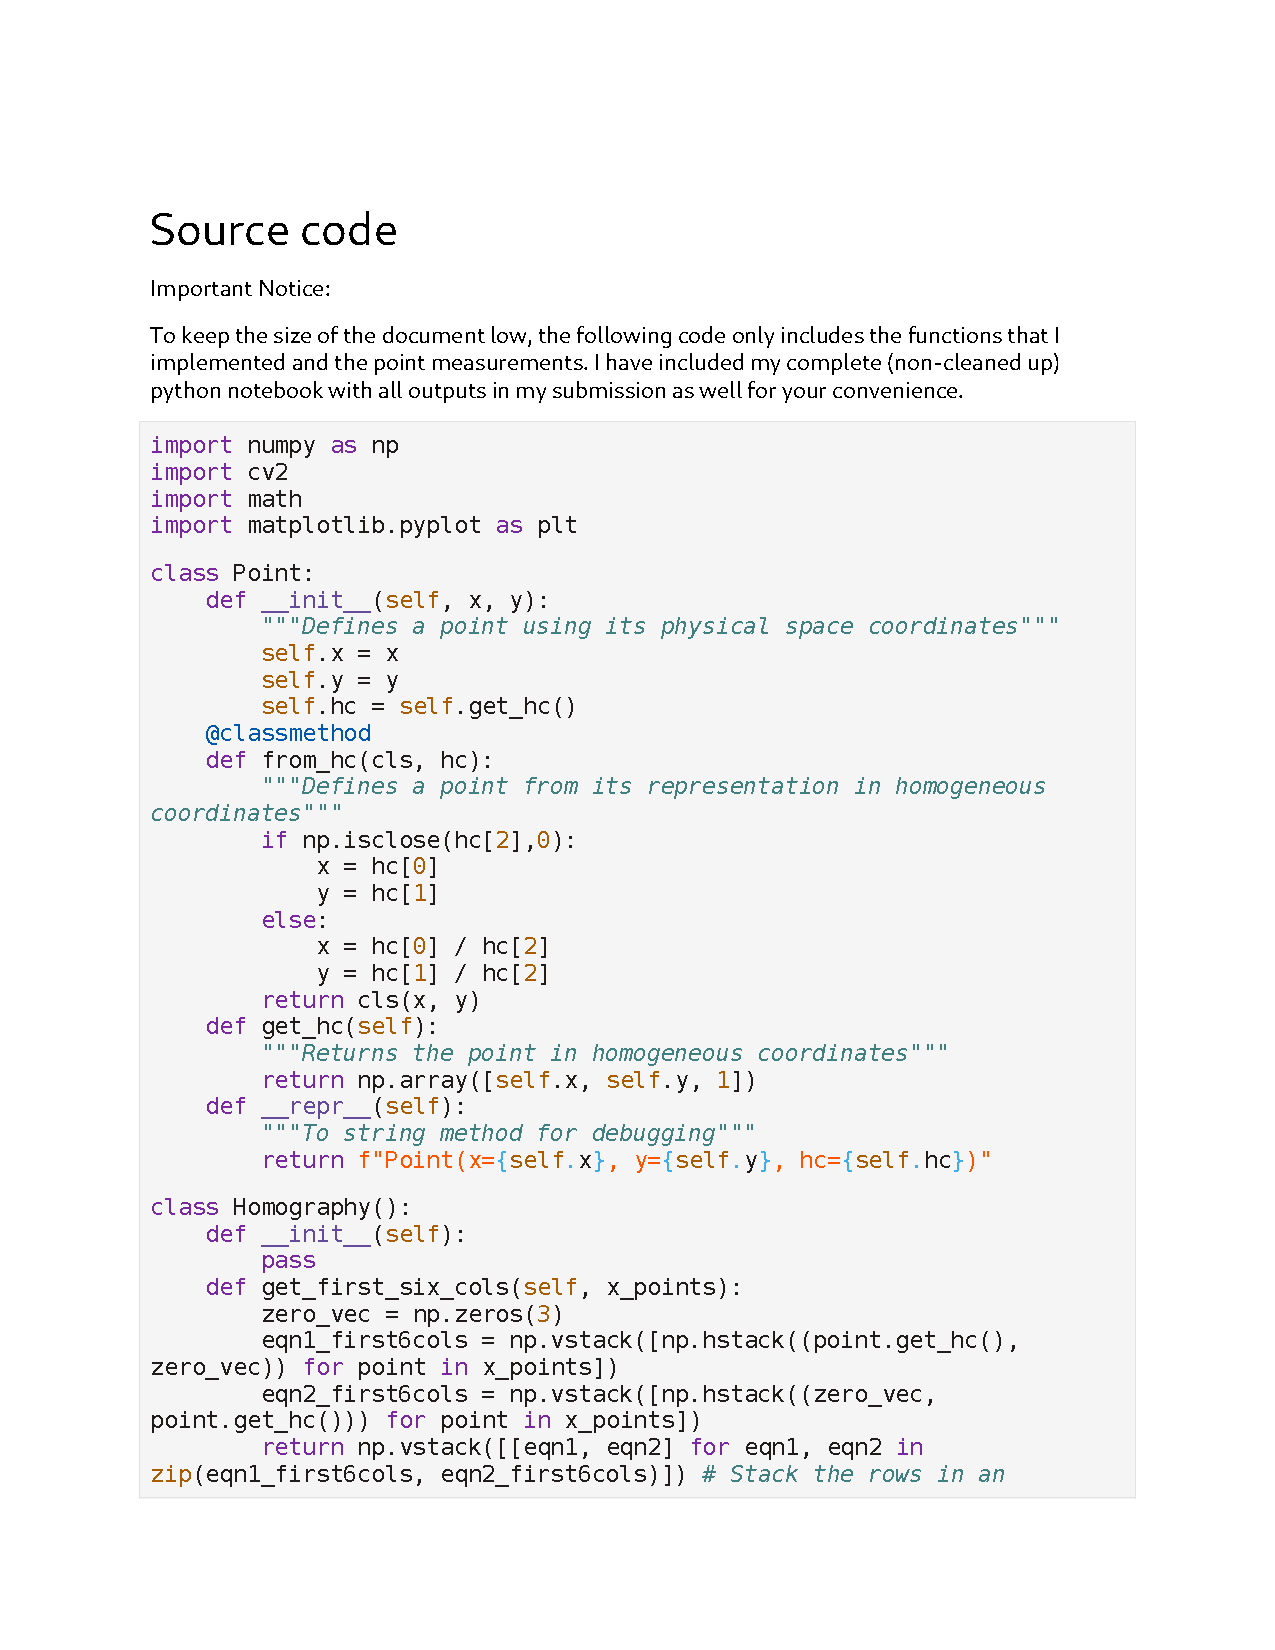
\includepdf[pages=-]{hw2.pdf}
\end{document}